% Created 2025-01-05 Sun 19:14
% Intended LaTeX compiler: lualatex
\documentclass[11pt]{article}
\usepackage{fontspec}
\usepackage{graphicx}
\usepackage{lilyglyphs}
\usepackage{graphicx}
\usepackage{longtable}
\usepackage{wrapfig}
\usepackage{rotating}
\usepackage[normalem]{ulem}
\usepackage{amsmath}
\usepackage{amssymb}
\usepackage{capt-of}
\usepackage{hyperref}
\usepackage[cm]{fullpage}
\usepackage[headheight=15pt, headsep=10pt, top=1in, bottom=1in, left=0.75in, right=0.75in]{geometry} % Ensure sufficient header space
\usepackage{fancyhdr}
\pagestyle{fancy}
\fancyhf{}
\fancyhead[L]{\textbf{ii-V-I Snippets}} % Left header with title
\fancyhead[R]{\textbf{Bartev - Lesson 26 (2024-12)}} % Right header with author
\fancyfoot[C]{\thepage}
\fancyfoot[R]{Printed \today} % Right footer with today's date
\renewcommand{\headrulewidth}{0.4pt} % Optional: Add a horizontal rule below the header
\makeatletter
\let\ps@plain\ps@fancy % Apply "fancy" style to the first page
\let\maketitle\relax % Suppress default title/author rendering
\makeatother
\author{Bartev}
\date{\today}
\title{ii-V Snippets}
\hypersetup{
 pdfauthor={Bartev},
 pdftitle={ii-V Snippets},
 pdfkeywords={},
 pdfsubject={},
 pdfcreator={Emacs 29.4 (Org mode 9.6.15)}, 
 pdflang={English}}
\begin{document}

\maketitle

\section*{Various chord changes}
\label{sec:orgaf51e64}

\subsection*{Major ii-V-I}
\label{sec:orgcd6efbb}
\begin{center}
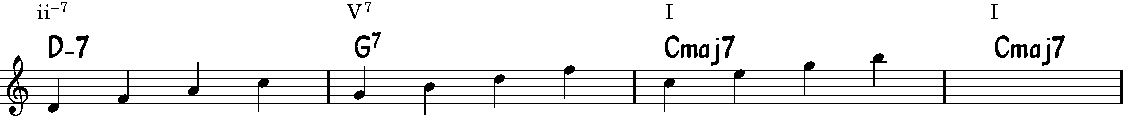
\includegraphics[width=.9\linewidth]{major_ii_v_i.pdf}
\end{center}

\subsection*{Minor ii-V-I}
\label{sec:org6b5d222}

\begin{center}
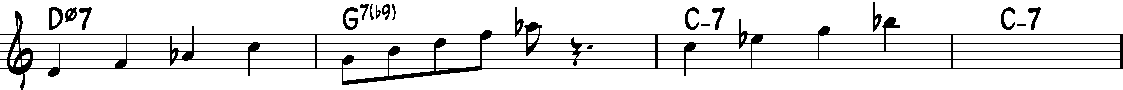
\includegraphics[width=.9\linewidth]{minor_ii_v_i.pdf}
\end{center}

For the half-dim chord, try the Locrian or Locrian nat 2 scales.

\begin{center}
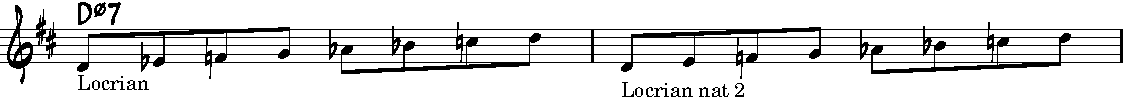
\includegraphics[width=.9\linewidth]{locrian.pdf}
\end{center}

For the G7\flat 9, try the Phrygian Dominant or altered scales.

\begin{center}
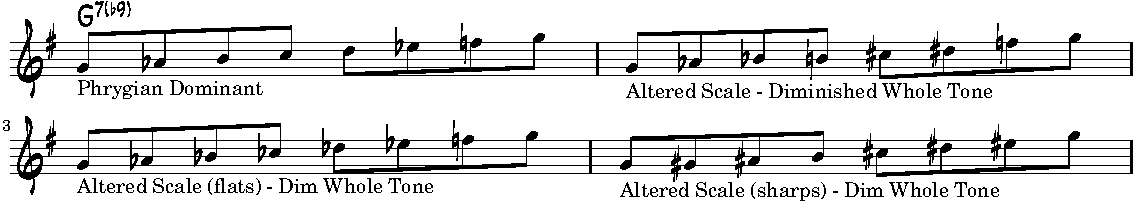
\includegraphics[width=.9\linewidth]{phryg_dom.pdf}
\end{center}

\section*{Basic ii-V-I phrases}
\label{sec:orgd56d203}
\subsection*{In E-flat}
\label{sec:orgeef5ef9}

Pellentesque dapibus suscipit ligula.  Donec posuere augue in quam.  Etiam vel tortor sodales tellus ultricies commodo.  Suspendisse potenti.  Aenean in sem ac leo mollis blandit.  Donec neque quam, dignissim in, mollis nec, sagittis eu, wisi.  Phasellus lacus.  Etiam laoreet quam sed arcu.  Phasellus at dui in ligula mollis ultricies.  Integer placerat tristique nisl.  Praesent augue.  Fusce commodo.  Vestibulum convallis, lorem a tempus semper, dui dui euismod elit, vitae placerat urna tortor vitae lacus.  Nullam libero mauris, consequat quis, varius et, dictum id, arcu.  Mauris mollis tincidunt felis.  Aliquam feugiat tellus ut neque.  Nulla facilisis, risus a rhoncus fermentum, tellus tellus lacinia purus, et dictum nunc justo sit amet elit.


\begin{center}
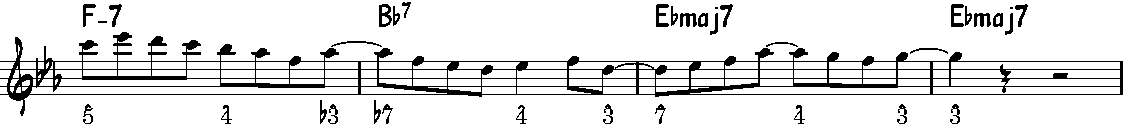
\includegraphics[width=.9\linewidth]{e-flat.pdf}
\end{center}

\subsection*{G maj}
\label{sec:org47061b7}
\begin{center}
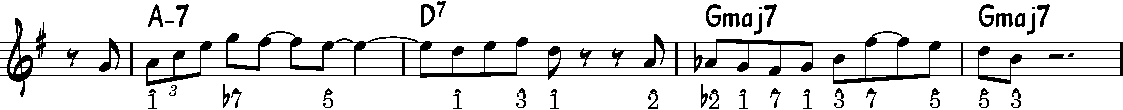
\includegraphics[width=.9\linewidth]{g_maj.pdf}
\end{center}

\subsection*{G maj (variation 2)}
\label{sec:org95abae9}
\begin{center}
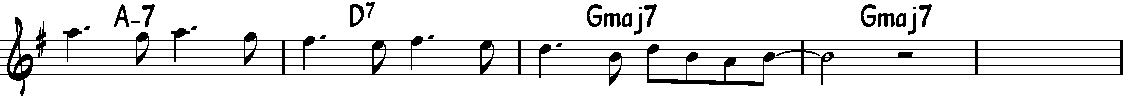
\includegraphics[width=.9\linewidth]{g_maj_v2.pdf}
\end{center}
\end{document}
